
\documentclass[11pt,a4paper]{article}
\usepackage[utf8]{inputenc}
\usepackage[T1]{fontenc}
\usepackage[french]{babel}
\usepackage{geometry}
\geometry{margin=1.8cm}
\usepackage{amsmath,amssymb}
\usepackage{graphicx}
\usepackage{booktabs}
\usepackage{array}
\usepackage{float}
\usepackage{xcolor}
\usepackage{hyperref}
\hypersetup{colorlinks=true,linkcolor=blue,urlcolor=blue}
\setlength{\parskip}{0.35em}
\setlength{\parindent}{0pt}

\title{\textbf{Projet de Recherche Opérationnelle}\\\large Routage, affectation, EOQ et méthode du simplexe}
\author{\textbf{Réalisé par :}\\[0.2cm]\begin{tabular}{ll}\textbf{C25936} & \textbf{MOHAMED CHERIV}\\\textbf{C30620} & \textbf{MOHAMEDEN ELBEDEWI}\end{tabular}\\[0.2cm]Module : Recherche Opérationnelle -- Licence}
\date{Année universitaire 2025--2026}

\begin{document}
\maketitle

\section*{Introduction}
La recherche opérationnelle propose des outils mathématiques pour améliorer la prise de décision lorsque les ressources sont limitées. Ce projet respecte les livrables demandés : rapport, code Python et présentation orale. Il étudie quatre applications complémentaires : un problème réel en Mauritanie, un problème universitaire, un problème de gestion de stock et une méthode fondamentale de programmation linéaire.

Les sujets retenus sont : le routage des camions d'eau dans les quartiers périphériques, l'affectation des étudiants aux projets, le dimensionnement de stock par le modèle EOQ, et la méthode du simplexe. Les trois premières applications répondent aux catégories demandées ; le simplexe est ajouté pour renforcer la partie fondamentale du projet.

Concernant les outils recommandés, le projet utilise \textbf{Python} avec \textbf{NetworkX} pour représenter le réseau de distribution sous forme de graphe pondéré. \textbf{NumPy} et \textbf{Matplotlib} sont utilisés pour les calculs numériques et les figures. Pyomo, PuLP ou OR-Tools sont des alternatives possibles pour des instances plus grandes, mais NetworkX est l'outil principal retenu ici car le routage est le cas algorithmique central du projet.

\section{Routage des camions d'eau}
\subsection*{Problématique}
Dans certains quartiers périphériques, l'eau peut être distribuée par camion. Le problème consiste à organiser les tournées pour satisfaire les points de distribution tout en minimisant la distance parcourue et en respectant la capacité du véhicule.

\begin{figure}[H]
\centering
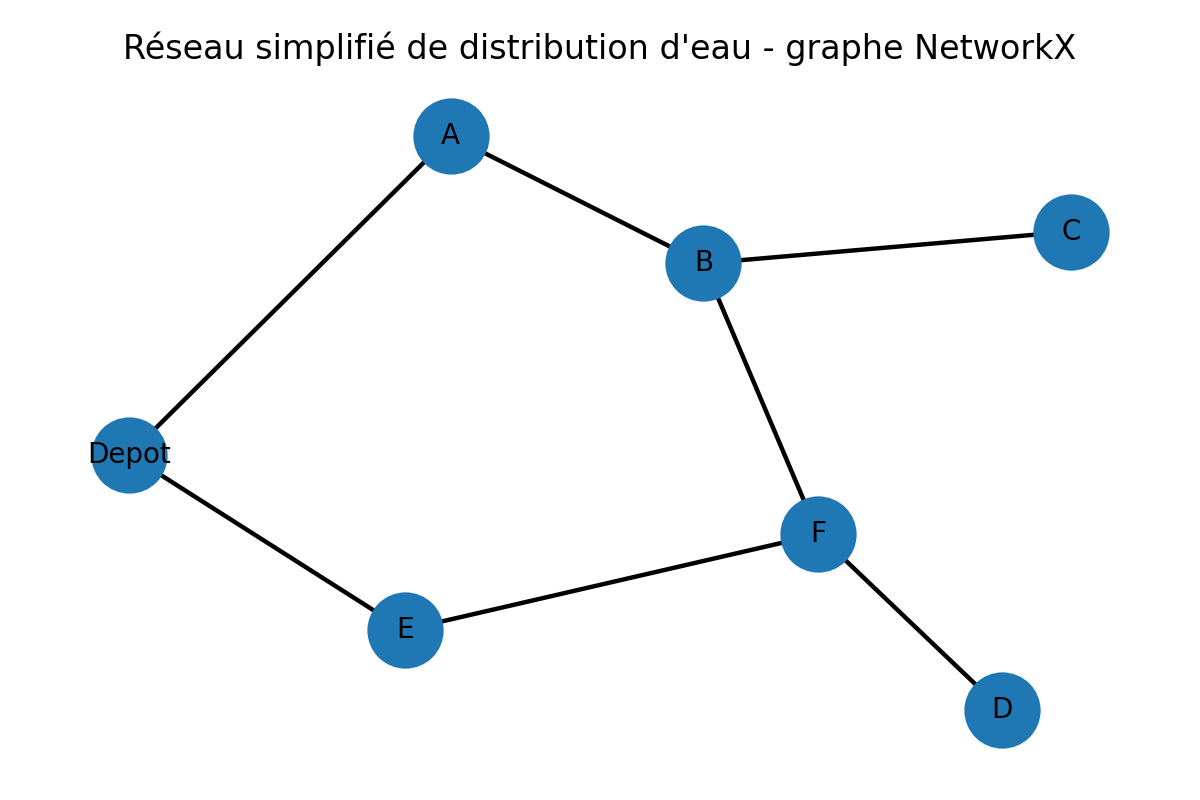
\includegraphics[width=0.65\textwidth]{figures/water_network.png}
\caption{Réseau simplifié de distribution d'eau.}
\end{figure}

\subsection*{Données et modèle}
On considère un dépôt central, six points de distribution et une capacité du camion de 1000 litres. Les demandes sont :

\begin{center}
\begin{tabular}{ccccccc}
\toprule
Point & A & B & C & D & E & F \\
\midrule
Demande (L) & 200 & 300 & 150 & 250 & 100 & 200 \\
\bottomrule
\end{tabular}
\end{center}

La demande totale vaut 1200 litres ; au moins deux tournées sont donc nécessaires. Les notations utilisées sont : $q_i$ pour la demande du point $i$, $Q$ pour la capacité du camion, et $d_{ij}$ pour la distance entre deux points. L'objectif est :
\[
\min Z = \sum d_{ij}x_{ij}
\]
avec $x_{ij}=1$ si le camion va de $i$ vers $j$, et $0$ sinon.

\subsection*{Méthode et résultat}
Le réseau est modélisé par un \textbf{graphe pondéré NetworkX} : les sommets représentent le dépôt et les points de distribution, et les arêtes représentent les distances. La méthode utilisée est une heuristique du plus proche voisin : le camion choisit à chaque étape le point non encore visité le plus proche, tant que sa capacité restante le permet. Les tournées obtenues sont réalisables et faciles à interpréter. Cette méthode n'assure pas toujours l'optimum global, mais elle donne rapidement une solution correcte pour une petite instance.

Les résultats générés par le script Python sont :
\begin{center}
\begin{tabular}{c p{7.8cm} c c}
\toprule
Tournée & Route & Charge & Distance \\
\midrule
1 & Dépôt--A--B--E--F--C--Dépôt & 950 L & 23 km \\
2 & Dépôt--D--Dépôt & 250 L & 14 km \\
\bottomrule
\end{tabular}
\end{center}
La distance totale obtenue est donc de 37 km.

\section{Affectation des étudiants aux projets}
\subsection*{Problématique}
Le deuxième problème consiste à affecter six étudiants à trois projets. Chaque projet a une capacité de deux étudiants. L'objectif est de maximiser la satisfaction totale en respectant les capacités.

\begin{figure}[H]
\centering
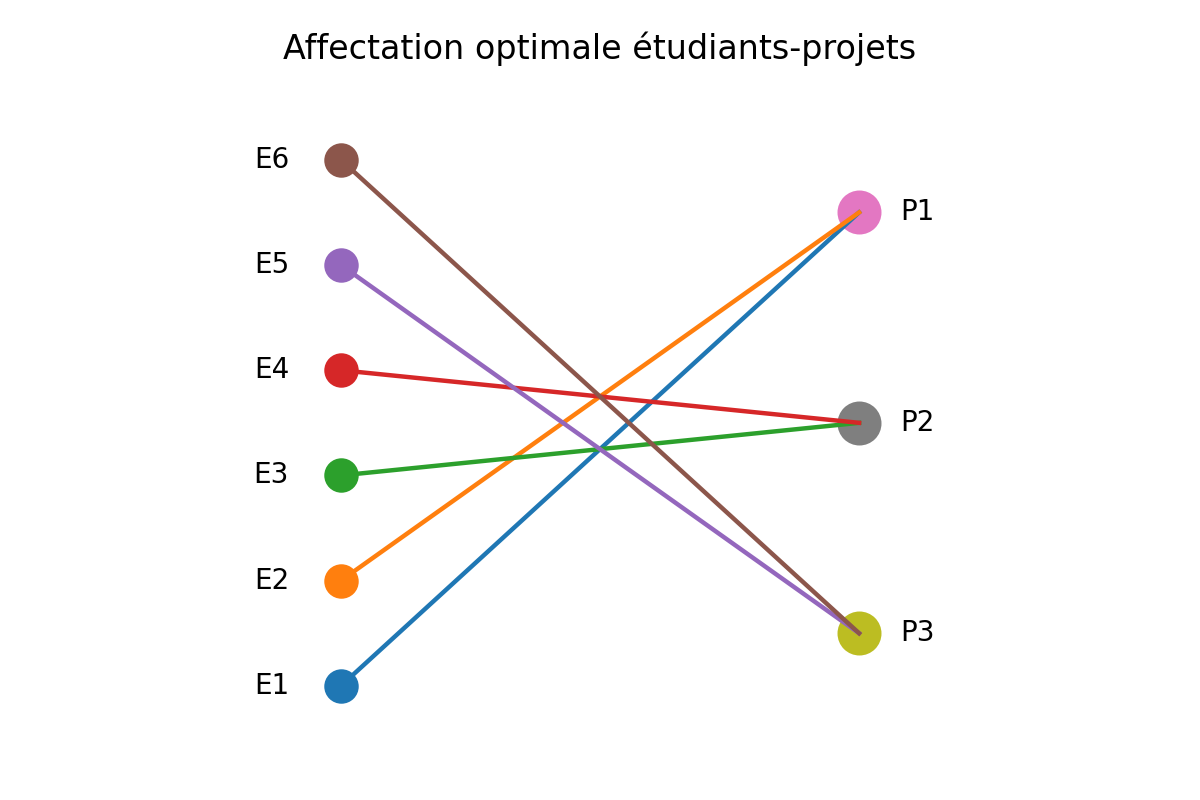
\includegraphics[width=0.62\textwidth]{figures/student_assignment.png}
\caption{Affectation optimale des étudiants aux projets.}
\end{figure}

\subsection*{Modèle mathématique}
La variable de décision est :
\[
x_{ij}=\begin{cases}
1 & \text{si l'étudiant } i \text{ est affecté au projet } j,\\
0 & \text{sinon.}
\end{cases}
\]
La fonction objectif est :
\[
\max Z = \sum_{i=1}^{6}\sum_{j=1}^{3}p_{ij}x_{ij}
\]
où $p_{ij}$ représente la préférence de l'étudiant $i$ pour le projet $j$.

Les contraintes sont :
\[
\sum_{j=1}^{3}x_{ij}=1 \quad \forall i
\]
\[
\sum_{i=1}^{6}x_{ij}=2 \quad \forall j
\]
\[
x_{ij}\in\{0,1\}
\]

\subsection*{Interprétation}
Le modèle garantit que chaque étudiant reçoit un seul projet et que chaque projet respecte sa capacité. La résolution exhaustive sur cette petite instance donne une affectation de satisfaction totale maximale.

\section{Dimensionnement de stock : modèle EOQ}
\subsection*{Problématique}
Le modèle EOQ (Economic Order Quantity) permet de déterminer la quantité économique de commande. Il équilibre le coût de commande et le coût de stockage.

Les données utilisées sont : $D=1200$ unités/an, $S=50$ MRU/commande et $H=2$ MRU/unité/an. La formule est :
\[
Q^* = \sqrt{\frac{2DS}{H}}
\]
\[
Q^* = \sqrt{\frac{2\times 1200\times 50}{2}} \approx 245
\]
La quantité optimale est donc d'environ 245 unités par commande.

\begin{figure}[H]
\centering
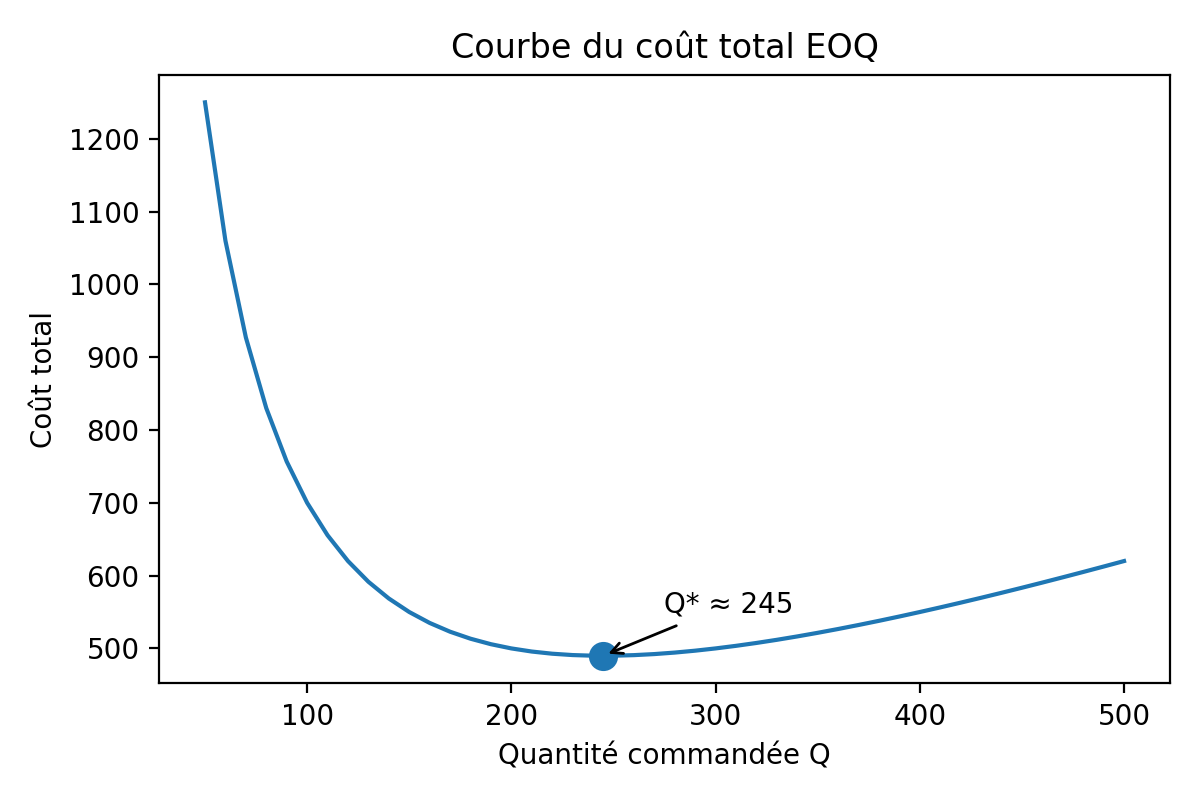
\includegraphics[width=0.62\textwidth]{figures/eoq_curve.png}
\caption{Minimum du coût total dans le modèle EOQ.}
\end{figure}

\section{Méthode du simplexe}
\subsection*{Problématique}
La méthode du simplexe est une méthode fondamentale pour résoudre les problèmes de programmation linéaire. Elle consiste à se déplacer d'un sommet admissible à un autre jusqu'à atteindre la solution optimale.

On étudie le problème suivant :
\[
\max z = 3x+4y
\]
Sous contraintes :
\[
x+2y\leq 8, \quad 3x+y\leq 9, \quad x,y\geq 0
\]

\subsection*{Mise sous forme standard}
On ajoute deux variables d'écart $s_1$ et $s_2$ :
\[
x+2y+s_1=8
\]
\[
3x+y+s_2=9
\]
Le tableau initial est :
\begin{center}
\begin{tabular}{c|ccccc}
\toprule
Base & $x$ & $y$ & $s_1$ & $s_2$ & RHS \\
\midrule
$s_1$ & 1 & 2 & 1 & 0 & 8 \\
$s_2$ & 3 & 1 & 0 & 1 & 9 \\
$z$ & -3 & -4 & 0 & 0 & 0 \\
\bottomrule
\end{tabular}
\end{center}

\subsection*{Résultat}
Après les pivots du simplexe, on obtient :
\[
x^*=2,\quad y^*=3
\]
\[
z^*=3(2)+4(3)=18
\]
Les deux contraintes sont saturées :
\[
2+2(3)=8, \quad 3(2)+3=9
\]

\begin{figure}[H]
\centering
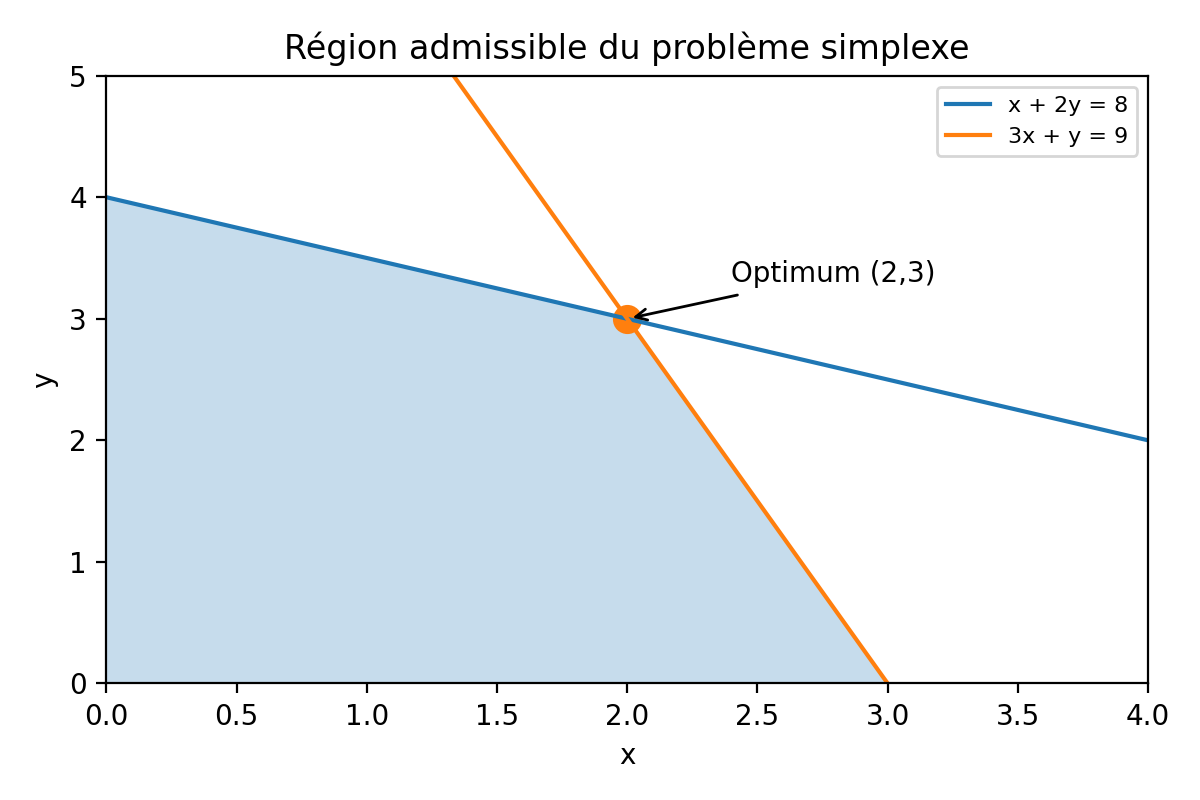
\includegraphics[width=0.62\textwidth]{figures/simplex_region.png}
\caption{Région admissible et solution optimale du simplexe.}
\end{figure}

\section{Comparaison des modèles}
\begin{center}
\begin{tabular}{p{4.1cm}p{4.2cm}p{4.1cm}}
\toprule
Sujet & Type de problème & Méthode utilisée \\
\midrule
Routage des camions d'eau & Routage / VRP simplifié & NetworkX + plus proche voisin \\
Affectation étudiants-projets & Optimisation binaire & Recherche exhaustive sur petite instance \\
EOQ & Gestion de stock & Formule analytique \\
Simplexe & Programmation linéaire & Pivots successifs \\
\bottomrule
\end{tabular}
\end{center}

\section*{Conclusion}
Ce projet montre que la recherche opérationnelle peut être appliquée à des problèmes différents : logistique locale, organisation universitaire, gestion de stock et programmation linéaire classique. Le routage réduit les distances de livraison avec un graphe NetworkX, l'affectation améliore la satisfaction globale, EOQ réduit les coûts de stock, et le simplexe donne une solution optimale pour un modèle linéaire. La combinaison de ces sujets donne une vision pratique et théorique de la discipline.

\end{document}
